\section{Perancangan Antar Muka Aplikasi}
Sisi klien aplikasi \emph{question answering} yang akan dikembangkan dalam penelitian ini akan dibangun dengan menggunakan \emph{framework} AngularJS. Sistem memiliki satu buah halaman antar muka seperti terlihat pada Gambar \ref{fig:rancangan_antarmuka}. Masukan pertanyaan dan jawaban diletakkan dalam satu buah halaman yang sama. Pada tahap awal sebelum pengguna mengirimkan pertanyaan hanya akan disediakan sebuah \emph{field} dengan tipe \emph{text} dan sebuah tombol submit yang berfungsi untuk mengirimkan pertanyaan ke sever.

\begin{figure}[ht]
    \centering
    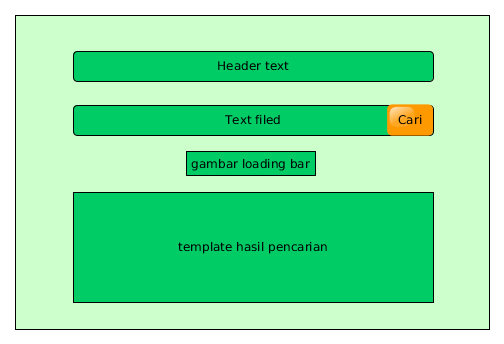
\includegraphics[width=1\textwidth]{bab_4/rancangan_antar_muka}
    \caption{Rancangan antar muka aplikasi \emph{question answering} data kabupaten di Nusa Tenggara Barat}
    \label{fig:rancangan_antarmuka}
\end{figure}

Bagian header berisi nama dari aplikasi sistem \emph{question answering} yang akan dibangun. Form pencarian diletakkan tepat di bawah header yang terdiri dari satu sebuah \emph{text field} yang digunakan untuk memasukkan pertanyaan serta sebuah tombol untuk melakukan submit pertanyaan. Atribut \emph{placeholder} dari \emph{input field} diisi dengan tulisan ``Masukkan pertanyaan'' untuk memudahkan pengguna memahami bagian \emph{input field} itu sendiri. Selanjutnya, di sebelah \emph{input field} terdapat sebuah tombol yang digunakan untuk melakukan submit form.

Bagian bawah \emph{input form} diletakkan sebuah gambar ``loading bar'' yang berfungsi untuk memberitahukan kepada user bahwa proses pencarian jawaban sedang berlangsung. Gambar ini akan muncul ketika pengguna telah melakukan submit form dengan cara menekan tombol ``cari'' atau dengan menekan tombol ``enter'' pada keyboard. Setelah jawaban diperoleh, maka gambar tersebut akan secara otomatis hilang dan jawaban hasil pencarian akan ditampilkan dibawahnya. Setelah jawaban ditampilkan, \emph{input field} tidak akan dikosongkan, hal ini dimaksudkan agar pengguna dapat melihat relasi antara pertanyaan yang dimasukkan dengan hasil jawaban yang didapatkan.

Tampilan jawaban terdiri dari dua bagian yaitu pada bagian atas akan ditampilkan rangkuman jawaban dan diikuti oleh data yang berasal dari objek ``inferedFacts'' yang dikirimkan oleh server. Data ``inferedFacts'' akan disajikan dalam bentuk tabel dengan nama properti di sebelah kiri dan isi dari properti di sebelah kanan.
